\documentclass{cslthse-msc}
\usepackage[utf8]{inputenc}
\usepackage[english]{babel}
\usepackage{amsmath}
\usepackage{amsfonts}
\usepackage{amssymb}
\usepackage{amsthm}
%\usepackage{makeidx}
\usepackage{graphicx}
\usepackage[titletoc, header, page]{appendix}

\usepackage{hyperref}
\usepackage{pdfpages}
\usepackage{rotating}
\usepackage{enumitem}
\usepackage{subfig}
\usepackage{float}
\usepackage{listings}
%% listings-modelica.cfg
%% Copyright 2014 Martin Sjoelund, Dietmar Winkler
%
% This work may be distributed and/or modified under the
% conditions of the LaTeX Project Public License, either version 1.3
% of this license or (at your option) any later version.
% The latest version of this license is in
%   http://www.latex-project.org/lppl.txt
% and version 1.3 or later is part of all distributions of LaTeX
% version 2005/12/01 or later.
%
% This work has the LPPL maintenance status `maintained'.
%
% The Current Maintainer of this work is Dietmar Winkler
%
% Code repository https://github.com/modelica-tools/listings-modelica
%
% This work consists of the file listings-modelica.cfg

\lstdefinelanguage{modelica}
{
  morekeywords=[1]{
    algorithm,and,annotation,as,assert,block,break,case,class,connect,connector,
    constant,constrainedby,der,discrete,each,else,elseif,elsewhen,encapsulated,
    end,enumeration,equality,equation,expandable,extends,external,failure,final,
    flow,for,function,guard,if,import,in,initial,inner,input,List,local,loop,
    match,matchcontinue,model,not,operator,Option,or,outer,output,package,parameter,
    partial,protected,public,record,redeclare,replaceable,return,stream,
    subtypeof,then,Tuple,type,uniontype,when,while},
  morekeywords=[2]{true, false},
  % Do not make true,false keywords because fn(true,x, false ) shows up as fn(true,x, *false*)
  sensitive=true,
  comment=[l]//,
  morecomment=[s]{/*}{*/},
  alsodigit={.,-},
  morestring=[b]',
  morestring=[b]",
}[keywords,comments,strings]

\definecolor{keywordcolor1}{rgb}{0,0,.4}
\definecolor{keywordcolor2}{rgb}{.90,0,0}
\definecolor{stringcolor}{rgb}{0.133,0.545,0.133}
% \definecolor{listingbgcolor}{rgb}{0.95,0.95,0.95}

\lstset{
  breaklines=true,
  language=modelica,
  basicstyle=\ttfamily,
  keywordstyle=[1]\color{keywordcolor1}\bfseries,
  keywordstyle=[2]\color{keywordcolor2},
  stringstyle=\color{stringcolor},
%  backgroundcolor=\color{listingbgcolor},
  framexleftmargin=5pt,
  xleftmargin=5pt,
  xrightmargin=5pt,
  showstringspaces=false
}

\newcommand{\code}[1]{\lstinline|#1|}
\newcommand{\modelica}[1]{\lstinline[language=modelica]|#1|}


%\geometry{showframe}

\author{
	Erik Hedblom \\
	{\normalsize \href{mailto:hedblom.e@gmail.com}{\texttt{hedblom.e@gmail.com}}}
	\and
	Kasper Rundquist \\
	{\normalsize \href{mailto:kasper.rundquist@gmail.com}{\texttt{kasper.rundquist@gmail.com}}}
}

\title{Safe regression test selection using static analysis}
%\subtitle{A {\LaTeX} class}
\company{Modelon AB}
\supervisors{Johan Ylikiiskilä, \href{mailto:johan.ylikiiskila@modelon.com}{\texttt{johan.ylikiiskila@modelon.com}}}{Jonatan Kämpe, \href{mailto:jonathan.kampe@modelon.com}{\texttt{jonathan.kampe@modelon.com}}}{Niklas Fors, \href{mailto:niklas.fors@cs.lth.se}{\texttt{niklas.fors@cs.lth.se}}}%\supervisor{Niklas Fors, \href{mailto:niklas.fors@cs.lth.se}{\texttt{niklas.fors@cs.lth.se}}}
\examiner{Görel Hedin, \href{mailto:gorel.hedin@cs.lth.se}{\texttt{gorel.hedin@cs.lth.se}}}

\date{\today}
%\date{January 16, 2015}

\acknowledgements{
If you want to thank people, do it here, on a separate right-hand page. Both the U.S. \textit{acknowledgments} and the British \textit{acknowledgements} spellings are acceptable.
}

\theabstract{
This document describes the Master's Thesis format for the theses carried out at 
the Department of Computer Science, Lund University. 

Your abstract should capture, in English, the whole thesis with focus on the problem and solution in 150 words. It should be placed on a separate right-hand page, with an additional \textit{1cm} margin on both left and right. Avoid acronyms, footnotes, and references in the abstract if possible.

Leave a \textit{2cm} vertical space after the abstract and provide a few keywords relevant for your report. Use five to six words, of which at most two should be from the title.
}

\keywords{Test Selection, Modelica}

\divisionoflabor{
}

%% Only used to display font sizes
\makeatletter
\newcommand\thefontsize[1]{{#1 \f@size pt\par}}
\makeatother
%%%%%%%%%%


\begin{document}
\makefrontmatter
\chapter[Introduction]{Introduction}

\section{Motivation / Background}
During software development, when a change is integrated into a project all previous testing have to be rerun. Test suites usually accumulates over time and regression testing can therefore be very time consuming. Depending on the change some or most of the test may be unrelated to the change and by excluding unrelated tests significant time savings could be achieved. ~\cite{DUMMY}


Det är viktig att testa mjukvara under utvecklingen för säkerställa att mjukvaran fungerar korrekt. När mjukvaran uppdateras måste testfall som redan testats utföras igen för att kontrollera att allt som fungerade innan uppdatering fortfarande fungerar efter. Det kan vara väldigt tidskrävande att köra samtliga test. Det finns därför mycket tid att spara om det går att utesluta test som garanterat inte har påverkas. För språket Modelica finns det inget verktyg för detta och det är därför intressant att utveckla ett.

\section{Problem Description / Aim / Goal}

The aim of this project is too reduce testing times for Modelica projects without loss of quality. This will be done by developing and implementing a method to exclude tests in a test suite unaffected by a specific change. Regression testing can then be performed with a reduced test suite without compromising quality.

\section{Regression Testing}
Regression tests are used to make sure that regression dose not occur. Software regression is when something that did work before do not work as expected due to a change.

\chapter[Background]{Background}
\section{Test Selection}
\begin{itemize}
	\item What is test selection?
	\item Different approaches
\end{itemize}
A safe Regression Test Selection (RTS) method will select all tests that produce a new result after a specific change. A safe RTS method is equivalent to running all tests. For a RTS method to be useful the RTS algorithm should run in less time than it takes to run the excluded tests. This is not necessary for each run, on average the overhead needs to be less than the time it takes to run the excluded tests.

There is a trade of between the precision of the test selection and the overhead. If a RTS algorithm has full precision it doesn't select any tests that can't fail. But the higher precision the more complex algorithm is needed. For a more complex algorithm its harder to follow the rules and verify that the RTS method is safe. A more complex algorithm also creates more overhead.

\section{Compiler}
\begin{itemize}
	\item SourceTree, InstanceTree, FlatTree
\end{itemize}
JModelica is an open source compiler that is developed and maintained by Modelon. OPTIMICA Compiler Toolkit is the commercial version of JModelica.

\section{Model Testing Toolkit}
Model testing Toolkit, MTT is a model testing toolkit that's going to use the test selection, MTT calls the OPTIMICA Compiler Toolkit where the dependency analysis is implemented.

MTT is based on nose tests for Python \cite{noseDoc}. Nose finds all tests automatically and runs them if nothing is specified. In MTT a test case is represented by a xml file and every test case has a Modelica model. So when you like to run test cases only associated with a specific model it's easy to select only the test cases which have the model you are interested in. When tests are run in MTT a HTML report of the results are created.

\section{Modelica}
\begin{itemize}
	\item What is Modelica?
	\item How can we perform test selection for Modelica?
	\end{itemize}

Modelica is an declarative, object oriented programming language where models are described by equations. It's used to get high performance simulations.

\subsection{Classes}
Basically everything in Modelica is classes. Built in types such as Integer are Modelica classes. Packages, models and functions are classes. Modelica is an object-oriented language, inheritance is possible. The extends clause is used to create an subclass of an superclass. In figure \ref{fig:classDefinition}, P2 is a subclass to P1, which is a superclass to P2. The subclass inherits everything in the superclass. The subclass may have more content than the superclass, but all the content in the super class is also in the subclass. 

\begin{figure}[H]
    \centering
    \subfloat{{\lstinputlisting[language=modelica]{modelica/packageDecl.mo}}}
    \caption{Class definition}
    \label{fig:classDefinition}
\end{figure}

A redeclare can be used to replace the declaration of an class or component with a new declaration. A component is a variable or an instance of a class. In figure ~\ref{fig:redeclare}, x is declared in model A. An instance of A is created in model C where x is redeclared. The y in model B, B.y, will have the value 1, while the y in model C, C.y, will have the value 2.

\begin{figure}[H]
	\lstinputlisting[language=modelica]{modelica/redeclare.mo}
    \caption{Redeclare}
    \label{fig:redeclare}
\end{figure}

\subsection{Name lookup}
In order to find a match for a name, Modelica starts by looking at the first name in a qualified name. Take for example the fully qualified name Modelica.Fluid.Pipes.StaticPipe. In this example Modelica is the first name in the qualified name.
\begin{itemize}
\item To find a match for the name, Modelica first checks if it's a built in type. If it's a built in type Modelica has found a match for the name.

\item If it's not a built in type Modelica looks in the class where the name is used, including inherited definitions, for a nested definition of the name. 

\item If there is no nested definition of the name, Modelica looks in the imports in the class where the name is used, inherited imports are not included, to find a match for the name.

\item If a match for the name is not found in the imports, Modelica looks for a nested definition in the enclosing package, including inherited definitions.

\item If the definition of the name isn't found in the enclosing package, Modelica looks for a imported definition, not including inherited imports, in the enclosing package.
\end{itemize}
If a match for the name still not is found, Modelica continues by using the same method and looking in the enclosing packages enclosing package and so on until: the enclosing package has the encapsulated qualifier or a package is a root package, in which case it doesn't have an enclosing package. In the first case the search for the name terminates and in the second case Modelica searches for a match in root level packages.

The search is done in the same way for the first name in a qualified name and an unqualified name. An unqualified name doesn't contain a dot, an unqualified name consists of only one name. StaticPipe is an example of an unqualified name.

If a name is a part of a qualified name and isn't the first name in the qualified name, it must be a nested definition within the definition of the previous name in the qualified name. In the example Modelica.Fluid.Pipes.StaticPipe, Fluid must be a nested definition within Modelica.\cite{modelicamodelica, tillermodelica}

\subsection{Import}
Imports are possible in Modelica to refer to a class or component in another package that is not in the same enclosing package. To find an imported object Modelica looks at root packages, so the fully qualified name needs to be used in an import. An import creates an alias. In the import below HydralicConductance will be mapped to the fully qualified name Modelica.Fluid.Types.HydralicConductance.

\lstinputlisting[language=modelica]{modelica/import.mo}

Modelica offers the option to rename an import. Here an alias will be created where the name Conductance is mapped to the fully qualified name Modelica.Fluid.Types.HydralicConductance.

\lstinputlisting[language=modelica]{modelica/renamedImport.mo}

Modelica allows the use of wildcard imports. Using wildcards it isn't possible to rename the import. This wildcard import will create an alias for every definition in Modelica.Fluid.

\lstinputlisting[language=modelica]{modelica/wildcardImport.mo}

To avoid multiple imports and wildcard imports, an multiple definition import can be used, from Modelica specification 3.3 \cite{modelicamodelica}. This multiple definition import creates two aliases, one mapping HydralicConductance to Modelica.Fluid.Types.HydralicConductance and one mapping HydralicResistance to Modelica.Fluid.Types.HydralicResistance.

\lstinputlisting[language=modelica]{modelica/multipleDefinitionImport.mo}

\subsection{Accesses}

\section{JastAdd}
JastAdd is a system based on reference attribute grammars, for extensible implementation of compilers. An Abstract Syntax Tree (AST) is used to represent a program. Attribute Grammars is amethod for declerativly defining computations on an AST. A node in an AST can have a synthezied attribute or an inherited attribute. An attribue is defined by an equation. A synthezied attribyte is defined in the node, an inherired attribute is defined in an ancestor node. A JastAdd specification is used to create an object-oriented framework.~\cite{aakesson2008development}

Collection attributes are defined by partial definitions in a number of arbitrary nodes. A node that have a partial definition of a collection attribute contributes to the value of the collection attribute. A collection attribute is usually a set where the empty set is the initial value of the collection attribute. The contributors, the nodes that contributes to the collection attribute, can for example contribute by adding elements to the set.~\cite{magnusson2007extending}

\chapter[Dependency analysis]{Dependency analysis}

To build the dependency graph we have constructed a set of rules to determine what creates dependencies. Due to limitations in JModelica, mainly pertaining to the lookup of names in the source tree, the rules have been adjusted to work around these limitations. We hope to have time to fix the limitations to perform a better and more accurate dependency analysis. First we introduce the rules and then we will go on and explain and motivate each one.

\paragraph{Rules}
\begin{enumerate}
\item A class depends on all resolvable accesses within it.
\item A class depends on its encapsulating class. 
\item All resolvable accesses in the path of an access generates dependencies to the encapsulating class.
\item A class depends on all classes encapsulated by the accessed class.
\item Exception to rule 4: Rule 4 is not applicable to import statements. An import should not add dependences to classes not imported but the import.
\end{enumerate}


\begin{figure}[!htbp]
    \centering
    \subfloat{{\includegraphics[scale=0.8]{EPS-graphs/Parent.eps}}}
    \qquad
    \subfloat{\raisebox{3.2 cm}{\lstinputlisting[language=modelica]{modelica/Parent.mo}}}
    \caption{A class depends on its encapsulating class}
    \label{fig:parentGraph}
\end{figure}

The first rule is perhaps the most intuitive, if a class accesses another class there is also a dependency to that class. However, due to the limitations in JModelica not all accesses in a class can be follows and therefor not all dependencies from this rule can be created. We will later see how the other rules compensate for this. 

The next rule, rule 2, will create a dependency from a class to it's encapsulating class. An example can be found in figure \ref{fig:parentGraph}. In the example there is a constant \textit{k} defined in package \textit{A}. If another with the same name were to be added in in model \textit{B} the reference to \textit{k} in \textit{C} will change to refer to the new constant. Therefore we need a dependency from \textit{C} to \textit{B}.

In figure \ref{fig:parentGraph} we also expect rule 1 to create a dependency from \textit{C} to \textit{A} due to \textit{k} being located in \textit{A}. However, the access \textit{k} cannot be resolved and we will miss the dependency to \textit{A}. In this case we can see that rule 2 can compensate by adding an indirect dependency from \textit{C} to \textit{A}. 
If the constant k in package \textit{A} is changed it will affect model \textit{C}. Therefore we need a dependency from \textit{C} to \textit{A}. With rule number 1 we get dependencies from \textit{C} to \textit{B} and from \textit{B} to \textit{A}. So we have an indirect dependency from \textit{C} to \textit{A}.

Another way to think about rule 2 is to consider what happens if \textit{A} or \textit{B} is removed. The \textit{C} can no longer be accessed since the path to \textit{C} is broken. This will cause the compilation of C to fail.

\begin{figure}[!htbp]
    \centering
    \subfloat{{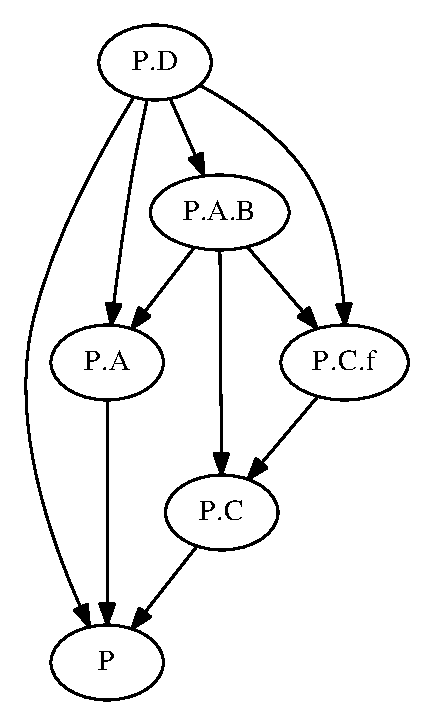
\includegraphics[scale=0.8]{EPS-graphs/DotAccess.eps}}}
    \qquad
    \subfloat{\raisebox{10 cm}{
        \begin{minipage}[t]{.5\textwidth}
        \centering
        \lstinputlisting[language=modelica]{modelica/DotAccess.mo}
        \end{minipage}}}
    \caption{Access with more access in its path, \textit{A.f}}
    \label{fig:dotAccess}
\end{figure}

In figure \ref{fig:dotAccess}, we want dependencies from model \textit{C} to all parts of the access to \textit{f}. This means that in addition to a dependency to \textit{f} a dependency to \textit{A} is also required. If package \textit{A} is removed it will cause a compilation error when model \textit{C} is compiled. This is caught by rule 3 and is why it is needed.


\begin{figure}[!htbp]
    \centering
    \subfloat{{\includegraphics[scale=0.8]{EPS-graphs/Component.eps}}}
    \qquad
    \subfloat{\raisebox{4.7 cm}{\lstinputlisting[language=modelica]{modelica/Component.mo}}}
    \caption{Access though component}
    \label{fig:component}
\end{figure}

Rule 4 is needed to handle the case in figure \ref{fig:component}. Ideally the access \textit{a.B.f} would create dependencies to \textit{A}, \textit{B} and \textit{f}. Because \textit{a} is a component, \textit{P.A.B.f} cannot be resolved and now dependencies can be created. Instead rule 4 is used to create to dependencies to everything defined in A when \textit{a} is declared.
It is also possible that an access can not be fully resolved. This is the case in \ref{fig:brokenAccess}, where the access \textit{P.a.f} cannot be resolved because the constant \textit{a} is a component. In this case the only resolvable part is \textit{P} and a  dependency is created to \textit{P} by rule 3. \textit{P} have dependencies to \textit{A} and \textit{f} through due to rule 4. Hence, it is not a problem that rule 4 cannot be applied to \textit{P.a.f}.

\begin{figure}[!htbp]
    \centering
    \subfloat{{\includegraphics[scale=0.8]{EPS-graphs/BrokenAccess.eps}}}
    \qquad
    \subfloat{\raisebox{4.7 cm}{\lstinputlisting[language=modelica]{modelica/BrokenAccess.mo}}}
    \caption{Access containing a component}
    \label{fig:brokenAccess}
\end{figure}

The exception to rule 4 is added to improve the precision of the test selection. Imports are specific and it is enough to add dependencies to what is actually imported. It is not uncommon to import packages located high up in the library structure. Without this exception unnecessary dependencies would be added to all or large part of the library. For example in Modelica's standard library there are several imports of Modelica, which is the top level package. Such import would create dependencies to every single class in the library. (Such imports may seem unnecessary and in fact they often are, but they can be used to affect the name lookup if there exists classes with the same name in the library)  



\subsection{Incremental updating}

\section{Test selection}

\chapter[Implementation]{Implementation}
We have implemented two different options for the dependency analysis, it can either be done based on files or Modelica classes. To do the dependency analysis and get an inverted dependency graph from the Modelica compiler, we specify which files or models that has changed. The dependency analysis are done for the specified Modelica classes or for all Modelica classes in the specified files. After the dependency analysis is done we invert the graph and returns a set of Modelica classes that may have changed.

If a class depends on something in, a library that aren't a part of any of the following: 
\begin{itemize}
	\item The library the class is in.
	\item The library any of the other specified classes are in.
	\item The library of, a class that are set to be included in the analysis
\end{itemize}
the dependency to that library is not included in the dependency graph. Lets look at an example where we specify that class P.A, in figure \ref{fig:libraryGraph}, has changed. Then P is the library A is in. A have a dependency to B in library MSL, here we will not include MSL.B in the dependency analysis and by that neither classes that MSL.B depends on. When we find a dependency to MSL.B we stops the analysis there.

\begin{figure}[H]
    \centering
    \subfloat{{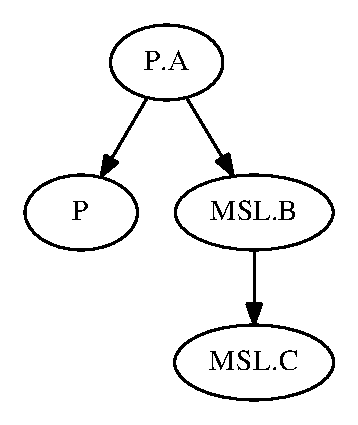
\includegraphics[scale=0.8]{EPS-graphs/LibraryExample.eps}}}
    \caption{Dependency graph}
    \label{fig:libraryGraph}
\end{figure}

Summary of approach:
\begin{itemize}
	\item Only do dependency analysis on given Modelica classes
	\item Don't continue the analysis in libraries that aren't specified
\end{itemize}
\section{Inverted dependency graph}
\begin{figure}[H]
    \centering
    \subfloat{{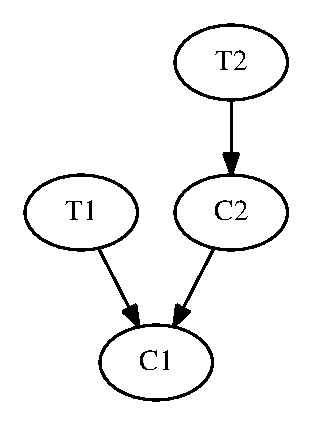
\includegraphics[scale=0.8]{EPS-graphs/GraphExample.eps}}}
    \caption{Dependency graph.}
    \label{fig:dependencyGraph}
\end{figure}
In the example above figure \ref{fig:dependencyGraph}, we have two Modelica classes, C1 and C2. C2 have a dependency to C1. We also have two tests, T1 and T2. T1 tests C1 and T2 tests C2. When C1 is changed both tests, T1 and T2 should be selected. When C2 is changed only test T2 needs to be selected.

When we specify that a class has changed, we want to get a set containing all classes that may be affected. So if we specify that C2 has changed, C2 is the only class that can be affected. If we instead say that C1 has changed both C1 and C2 may be affected. Starting from C1, the problem is to find all classes that depends on C1. To solve this we need to invert the dependency graph, in figure \ref{fig:dependencyGraph}, and then get the inverted dependency graph in figure \ref{fig:invertedGraph}. 
\begin{figure}[H]
    \centering
    \subfloat{{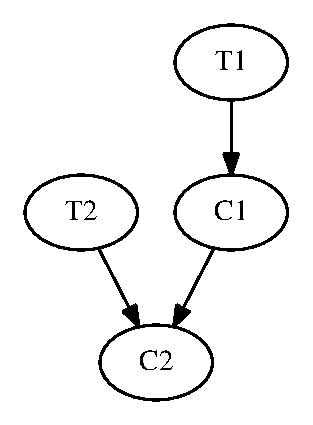
\includegraphics[scale=0.8]{EPS-graphs/InvertedGraphExample.eps}}}
    \caption{Inverted dependency graph.}
    \label{fig:invertedGraph}
\end{figure}
\section{External functions}
The Modelica language allows the use of external functions that are not defined in a Modelica file. The external functions are often defined in a C-file.\cite{modelicamodelica}

In our dependency analysis we can't analyze the dependencies in external files. To handle this, and keep the test selection safe, if a file that isn't a Modelica file has changed we assume that every Modelica class that has a reference to an external has changed.
\chapter[Evaluation]{Evaluation}
\begin{itemize}
	\item Savings
	\item Precision
\end{itemize}

\begin{figure}
    \centering
    \makebox[\textwidth][c]{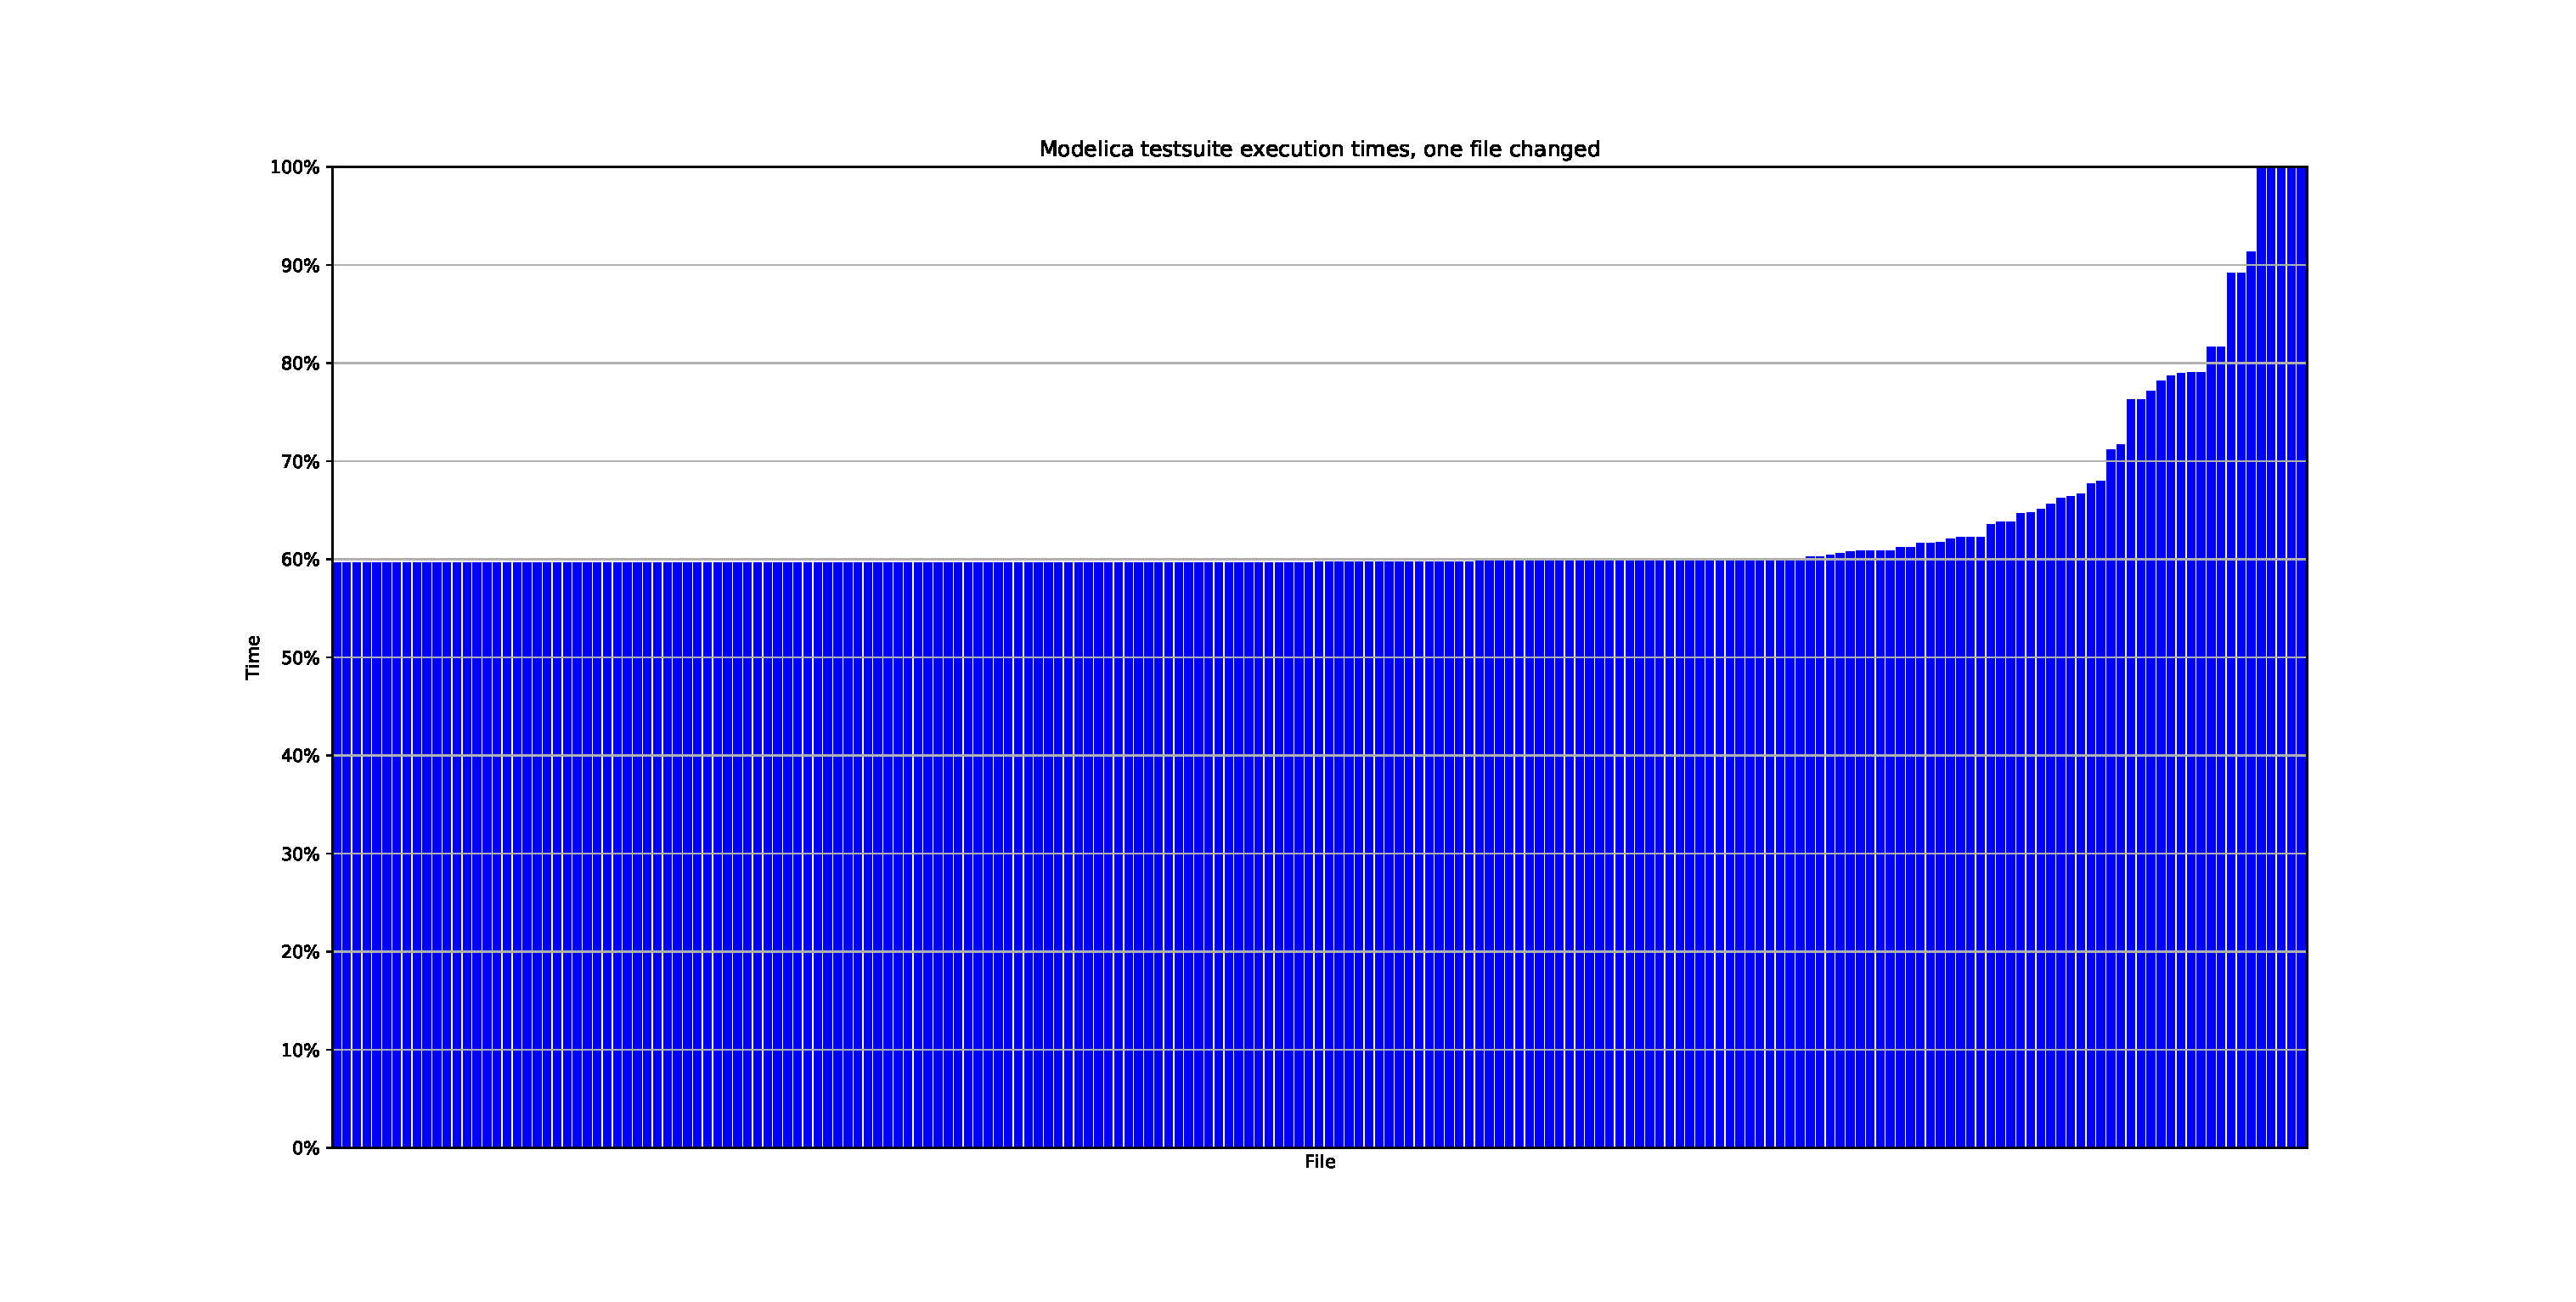
\includegraphics[width=1.5\textwidth]{EPS-graphs/one_file.eps}}
    \caption{One file changed.}
    \label{fig:onefile}
\end{figure}

\begin{figure}
    \centering
    \makebox[\textwidth][c]{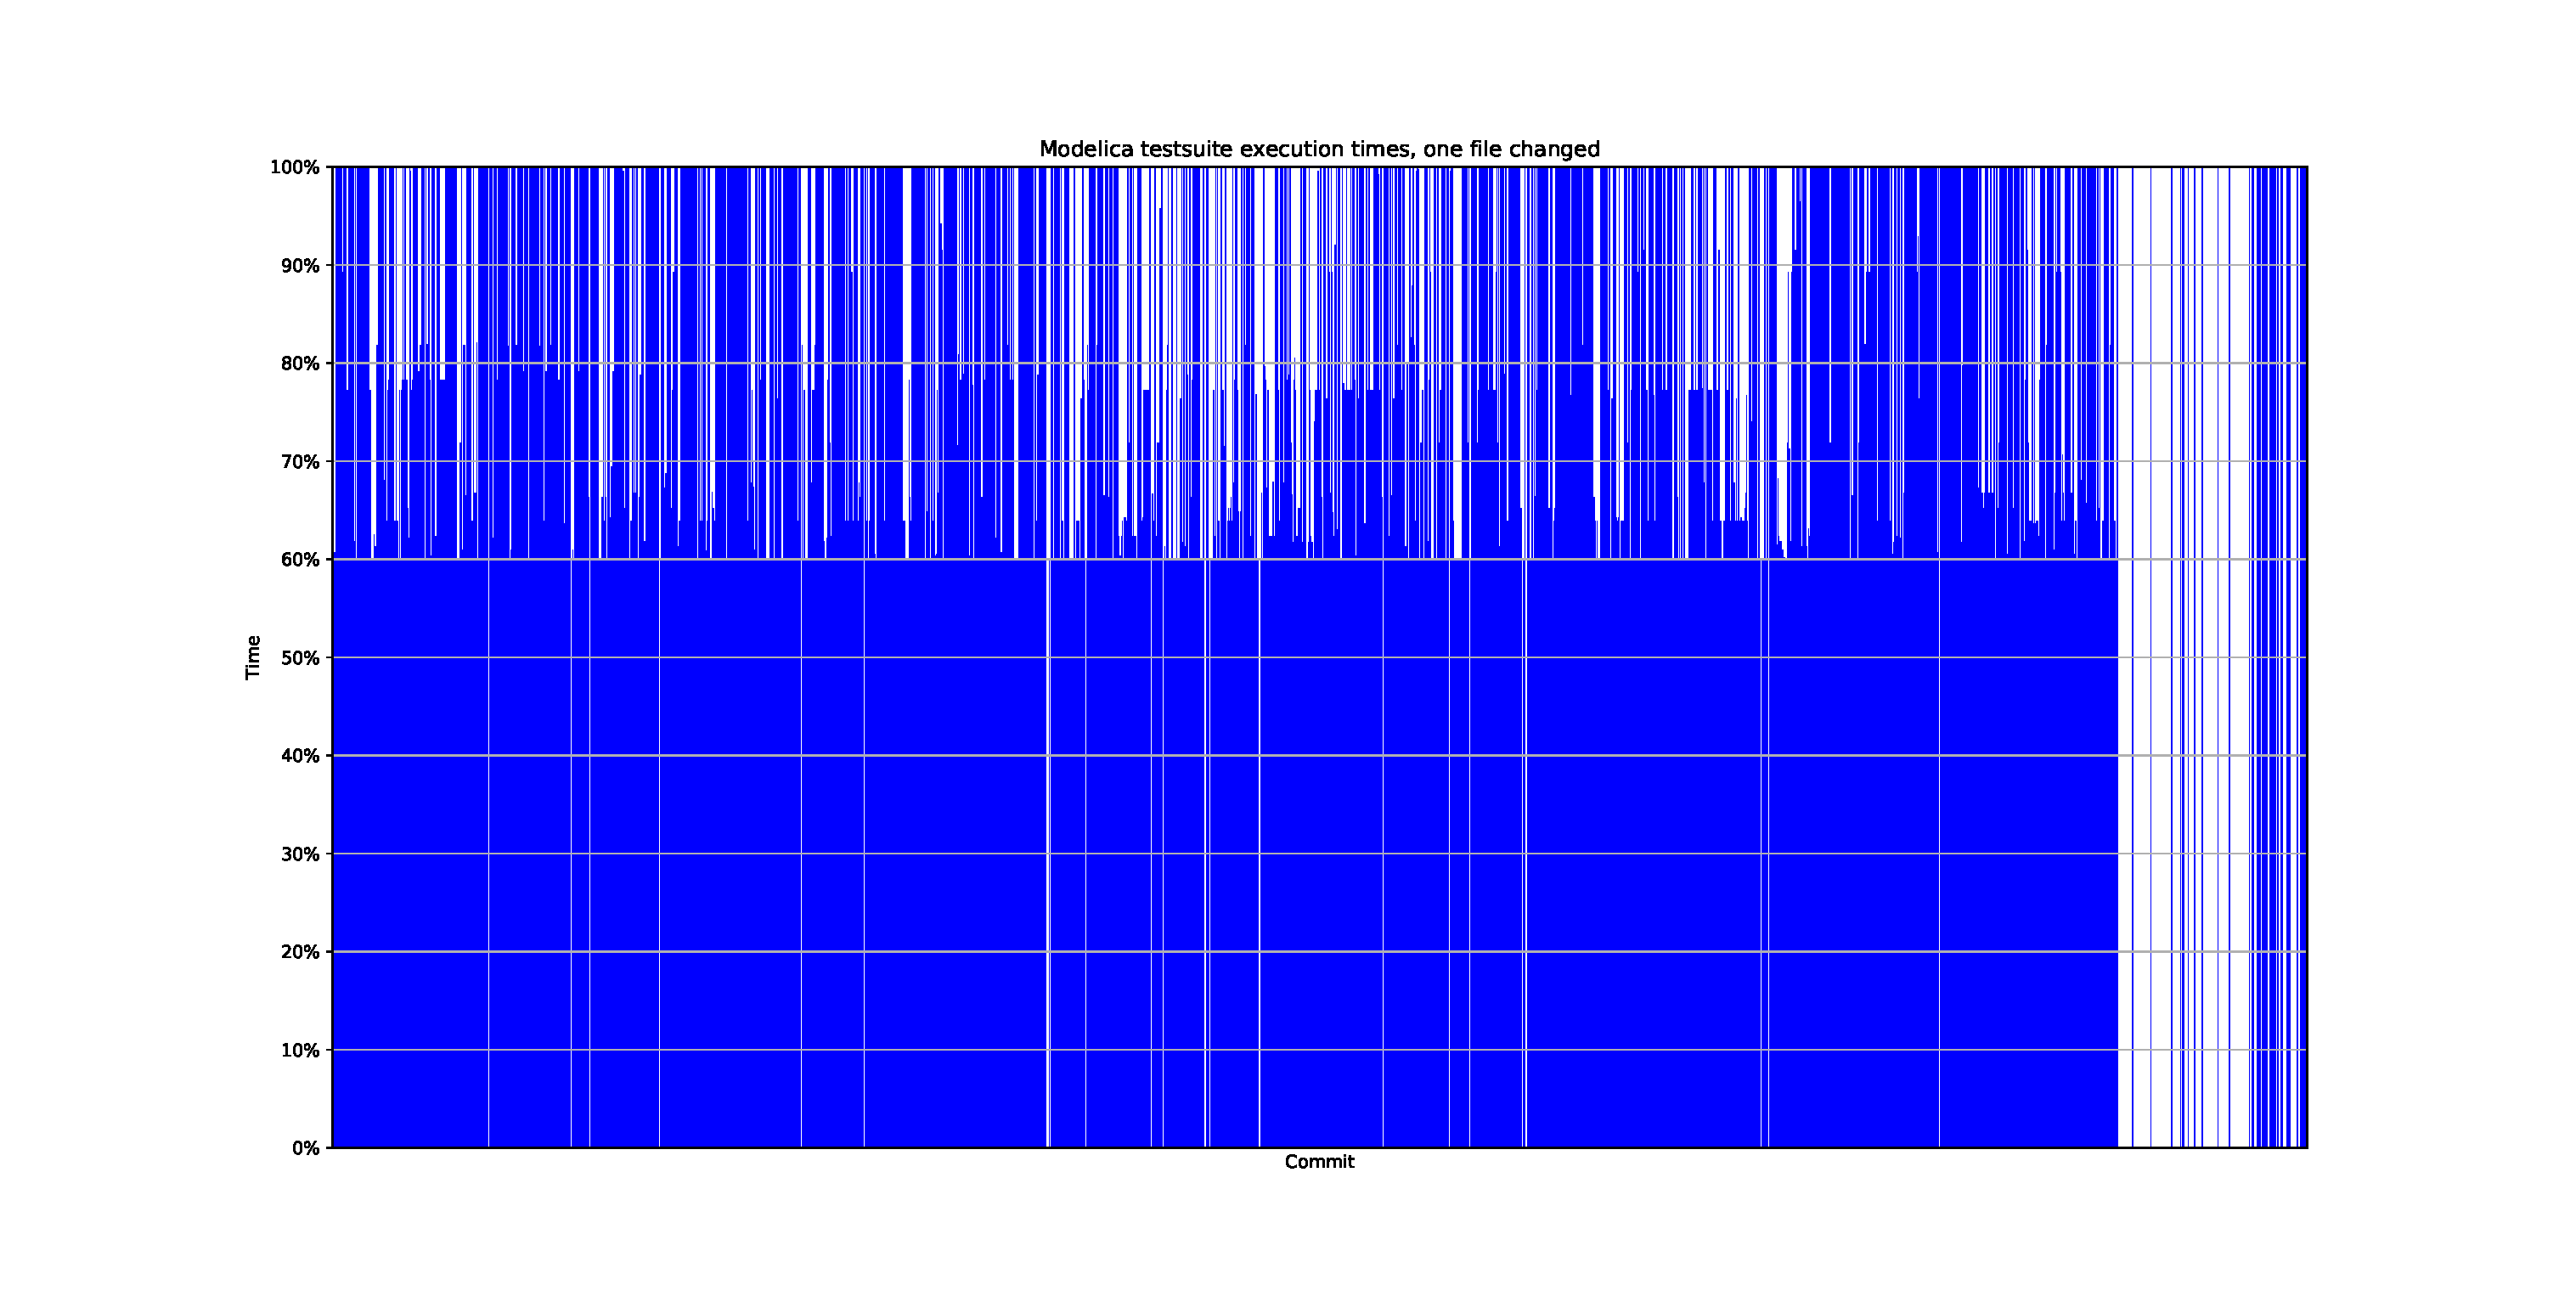
\includegraphics[width=1.5\textwidth]{EPS-graphs/history_plot.eps}}
    \caption{history plot for MSL.}
    \label{fig:mslhistory}
\end{figure}

\chapter[Future Work]{Future Work}
	
\chapter[Discussion]{Discussion}



\begin{itemize}
	\item Validity
	\item Analysis granularity
    \item Good and bad Modelica patterns for dependency analysis
\end{itemize}

\section{Related Work}

% Kan kanske flyttas till bakgrunden ev till test selection delen.
A master thesis similar to this one has previously been done at LTH. In the previously master thesis JastAdd was used to decrease the cost for testing of Android projects ~\cite{kampe2012dependroid}. There is research done on test selection. A method for safe RTS for Java has been developed before, that has many similarities with the method we are developing for Modelica. 

Studies have been conducted to investigate at which granularity dependency analysis pays off the most and how much percision it can have with out getting to expensive ~\cite{DBLP:conf/sigsoft/LegunsenHSLZM16}. It has also been done work in other techniques to achieve shorter time for testing, including dynamic test selection.

Det har tidigare gjorts ett liknande examensarbete på LTH. Där användes JastAdd för att minska kostnaden för testning av Android projekt. Det finns även forskning på området. Nästan precis samma sak som vi ska göra har gjorts tidigare men för Java ~\cite{DBLP:conf/pppj/OqvistHM16}. Utöver detta har det även tidigare undersökts hur finkornig en beroendeanalys kan vara utan att den blir för dyr ~\cite{DBLP:conf/sigsoft/LegunsenHSLZM16}. Det finns även arbete inom andra tekniker för att uppnå kortare test tider, till exempel dynamiskt testurval.
\chapter[Conclusion]{Conclusion}
\makebibliography{thebib}

\begin{appendices}
\chapter{About This Document}
\end{appendices}


\end{document}